\documentclass[a4paper,11pt]{book}
\newcommand{\Origin}{/home/ttt/Desktop/book/cfd-openfoam}

\usepackage{color}
\usepackage{layouts}
\usepackage{cclicenses}
\usepackage{morefloats}
\usepackage{paralist}
\usepackage{chngcntr}
\usepackage{layouts}
\usepackage{fancyhdr}
\pagestyle{headings}
\usepackage{amsmath,graphicx,makeidx}
\usepackage{fancybox,url}
\usepackage{cite}
%\usepackage{appendix}
\counterwithout{footnote}{chapter}
\usepackage{subfig}
\usepackage{listings}
\usepackage{varioref} % for \vref commands
%\usepackage{hyperref}

\newcommand{\redcolor}[1]{\color{red}#1\color{black}}
\newcommand{\codclr}{10pt}
\newcommand{\scilab}{Scilab}
\newcommand{\arduino}{Arduino Uno}
\newcommand{\ie}{\emph{i.e.},}

\newcommand{\ourname}[1]{\\ [1.5mm] \noindent{\bf #1}}
% Shroff book size
%\textheight 7.75in
\textheight 7.5in
\textwidth 5.5in
\evensidemargin 0.625in
\oddsidemargin 0.625in

\newcommand{\Home}{/home/ttt/Desktop/book/cfd-openfoam}

\newcommand{\tnfig}{0.3\linewidth}
\newcommand{\smfig}{0.45\linewidth}%0.42
\newcommand{\smfigp}{0.49\linewidth}%0.42
\newcommand{\lgfig}{0.65\linewidth}%0.65
\newcommand{\hgfig}{0.9\linewidth}

\renewcommand\bibname{References}

\newcommand{\figref}[1]{Fig.~\ref{#1}}
\newcommand{\figrefp}[1]{Fig.~\vref{#1}}
\newcommand{\tabref}[1]{Table~\ref{#1}}
\newcommand{\tabrefp}[1]{Table~\vref{#1}}
\newcommand{\chapref}[1]{Chapter~\ref{#1}}
\newcommand{\secref}[1]{Sec.~\ref{#1}}
\newcommand{\sciref}[1]{Scilab~Code~\ref{#1}}
\newcommand{\ardref}[1]{Arduino~Code~\ref{#1}}
\newcommand{\mypageref}[1]{Page~\pageref{#1}}
\newcommand{\fnref}[1]{Footnote~\ref{#1}}
\renewcommand{\topfraction}{1}
\renewcommand{\bottomfraction}{1}
\renewcommand{\textfraction}{0}
\renewcommand{\floatpagefraction}{1}
% \bibliographystyle{./IEEEtran}
\bibliographystyle{unsrt}

\hyphenation{Ashu-tosh pr-ess}

\makeindex
\begin{document}
\pagestyle{plain}
\pagestyle{empty}
\frontmatter
\thispagestyle{empty}
%\input{suppl/dedicate}
\pagestyle{headings}
\tableofcontents
\listoffigures
\listoftables
%\listofard
%\listofcode
%\thispagestyle{empty}
\addtocontents{toc}{\protect\thispagestyle{empty}}
%\input{suppl/preface}
%\input{suppl/acr}

\mainmatter
\pagestyle{headings}
\renewcommand\chaptermark[1]{\markboth{\bf {\thechapter. #1}}{}}
\renewcommand\sectionmark[1]{\markright{\bf {\thesection. #1}}}

%\input{texfiles/microcontintro.tex}
%\input{texfiles/sciaurint.tex}
%\input{suppl/intro.tex}
\chapter{Installing OpenFOAM and Paraview}
\thispagestyle{empty}
\label{sec:chap1}
\newcommand{\LocCHonefig}{\Origin/CHAPTERS/chap1/figures}

The First chapter deals with Installing OpenFOAM and Paraview. We are using Linux Operating System for installation and OpenFOAM-2.3.0 and Paraview-4.1.0.
First we will look how to install OpenFOAM and paraview using Synaptic Package Manager. Then using the downlading it from the OpenFOAM website and lastly installing
it using the source code. We will end this chapter with an example which shows running a simple problem in .As a basic requirement the user expected to have 
some basic knowledge of Computational Fluid Dynamics ( CFD ) and should be able to use basic Linux Commands.

\section{Installation using Synaptic Package Manager}

OpenFOAM and Paraview can be installed using Synaptic Package Manager. On the left side of your computer screen you can see the Launcher with the list of softwares.
Click on the search box ,Fig.\ref{search} on top of the Launcher and type Synaptic. This will display the Synaptic Package Manager. Click on it to open.

\begin{figure}[h]  
\begin{center}  
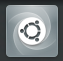
\includegraphics[scale=0.75]{\LocCHonefig/dash.png}
\caption{Search Icon on top of Launcher}
\label{search}
\end{center}  
\end{figure}

\flushleft You will be interrupted to enter the system password.

\begin{figure}[h]  
\begin{center}  
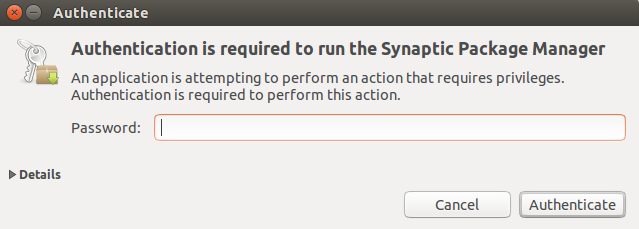
\includegraphics[scale=0.45]{\LocCHonefig/password.png}
\caption{Enter system password to open Synaptic Package Manager}
\end{center}  
\end{figure}
\vspace{1cm}

\flushleft Once the Synaptic Package Manager is Opened, in the search box type OpenFOAM.

\begin{figure}[ht]  
\begin{center}  
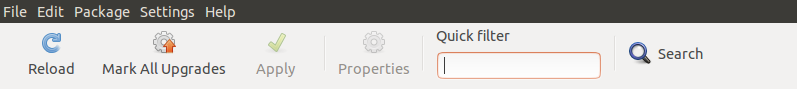
\includegraphics[scale=0.4]{\LocCHonefig/searchbox.png}
\caption{Search Box}
\label{searchbox}
\end{center}  
\end{figure}

\flushleft You will see both OpenFOAM-2.3.0 and Paraview-4.1.0. Right Click Both of them for installation and click Apply to install, Fig \ref{searchbox}. 
This might take some time to install depending upon your internet speed.

\begin{figure}[ht]  
\begin{center}  
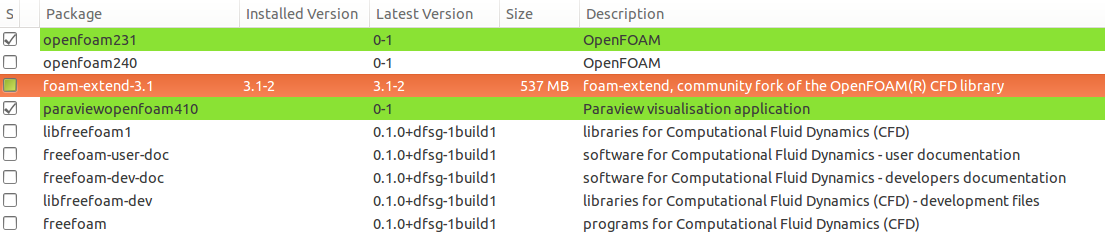
\includegraphics[scale=0.35]{\LocCHonefig/mark.png}
\caption{Install OpenFOAM and Paraview}
\label{searchbox}
\end{center}  
\end{figure}

\section{Installtion from OpenFOAM website}

\flushleft OpenFOAM can also be downloaded and installed using the OpenFOAM website. Follow the steps given below for installation. 
\begin{itemize}
\item On your browser type \textbf{www.openfoam.com/download} 
\item Go to Ubuntu Debian Installation
\item Under the first point of Installation copy the command line and paste this in your terminal window
\item Open the terminal window by pressing \textbf{Ctl+Alt+t} keys simultaneously on your keyboard or you can also open it using the 
search icon on top of the Launchbar

\begin{figure}[ht]  
\begin{center}  
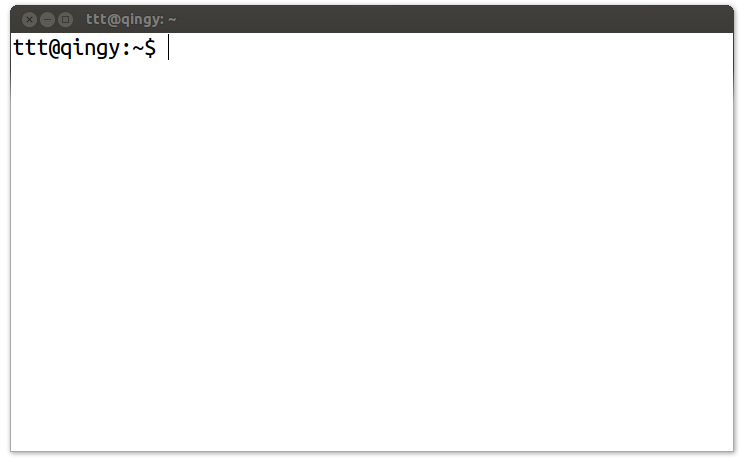
\includegraphics[scale=0.28]{\LocCHonefig/terminal.png}
\caption{Terminal window}
\label{terminal}
\end{center}  
\end{figure}

\item For complete installation for OpenFOAM and Paraview follow the steps under Ubuntu installation page

\end{itemize}

\flushleft To configure the installed software we need to edit the bashrc file. 
To do this open a new command terminal and type 
\begin{equation*}
\textbf{gedit $\sim$$\slash$.bashrc} 
\end{equation*}
and press enter

\flushleft After the bashrc file is opened scroll down to the bottom of the file. Then go back to your browser (OpenFOAM download page) and scroll down to \textbf{User Configuration}.  
Copy the line in point number 2  
\begin{equation*}
\textbf{source /opt/openfoam230/etc/bashrc} 
\end{equation*}
and paste it at the bottom of the bashrc file. Save it and close the file.

\flushleft To check if OpenFOAM is installed properly open a new command terminal and type 
\begin{equation*}
\textbf{icoFoam -help} 
\end{equation*}
and press enter. You will see a "Usage" message on your terminal screen, Fig \ref{usage} which shows that the installation is done.

\begin{figure}[ht]  
\begin{center}  
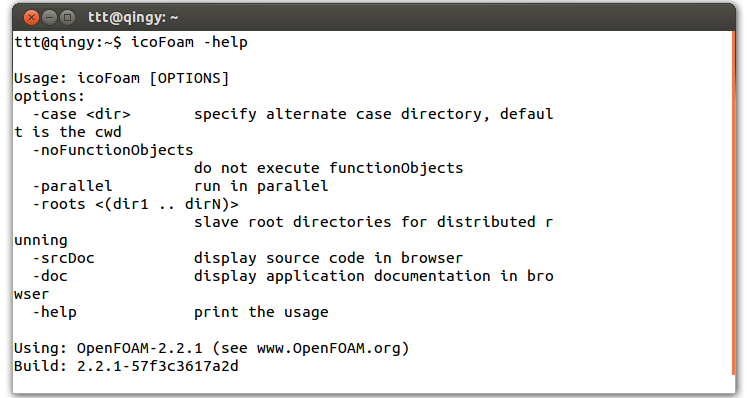
\includegraphics[scale=0.5]{\LocCHonefig/usage.png}
\caption{Usage Message}
\label{usage}
\end{center}  
\end{figure}

\flushleft Now we will set up the working directory and copy the tutorial folder. Follow the steps given below. 
\begin{enumerate}
\item Open up a new terminal and type \textbf{mkdir -p $\$$FOAM$\_$RUN} and press enter
\item Now type \textbf{cp -r $\$$FOAM$\_$TUTORIALS} \textbf{$\$$FOAM$\textunderscore$RUN} and press enter. This will copy the tutorials folder into the run directory.
\end{enumerate}

\flushleft Installation of OpenFOAM using the Debian package is now complete. Similarly you can download it for other linux OS such as Fredora, OpenSUSE.

\section{Installation using Source Code}
Alternate way to install OpenFOAM and Paraview is by Compiling the Source code available under the header of \textbf{Source Pack} Installation on the OpenFOAM website. 
Download the tar files available in \textbf{OpenFOAM.tar.gz} and \textbf{ThirdParty.tar.gz} format. Create a folder in your Home directory by the name OpenFOAM and paste the tar files in that folder and Extract the files in that folder.
Follow the steps given on the OpenFOAM source pack installation page to complete the installation. Since we compile the source code it might take a few hours to complete.

\section{Example Problem - Lid Driven Cavity}
We will solve an problem here by the name Lid Driven Cavity. It is a two dimensional problem where the upper plate moves and other three sides of the plate are fixed / stationary, \ref{lid}. 
The solver we use here is icoFoam which is an Transient solver for incompressible flow.

\begin{figure}[ht]  
\begin{center}  
\includegraphics[scale=0.3]{\LocCHonefig/geometry1.png}
\caption{Lid Driven Cavity}
\label{lid}
\end{center}  
\end{figure}

In the terminal type the path given below :\newline

\small{cd OpenFOAM/OpenFOAM-2.3.0/run/tutorials/incompressible/icoFoam/cavity} \newline

\subsection*{Meshing the geometry}
We need to mesh the geometry. This can be done using the blockMesh utility of OpenFOAM. In the command terminal type \textbf{blockMesh} and press $<enter>$ which completes the meshing, Fig \ref{mesh}

\begin{figure}[ht]  
\begin{center}  
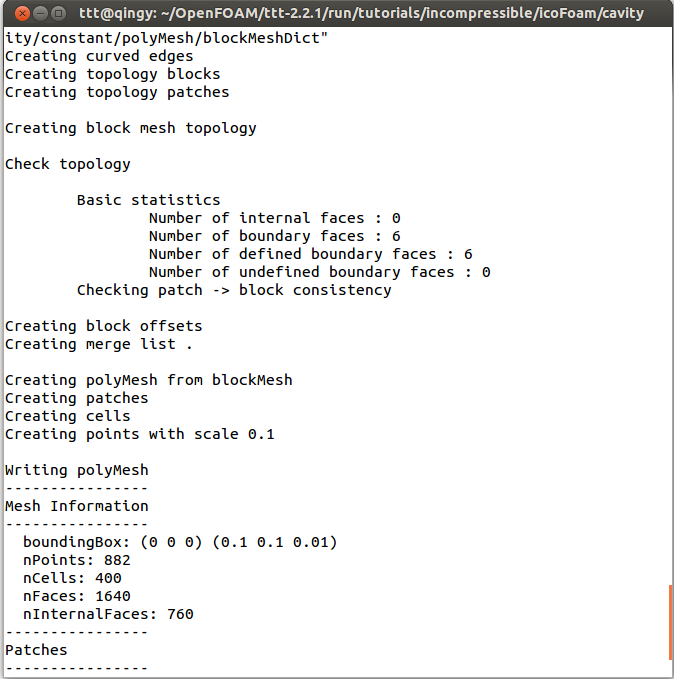
\includegraphics[scale=0.3]{\LocCHonefig/blockMesh.png}
\caption{blockMesh for meshing}
\label{mesh}
\end{center}  
\end{figure}

\newpage

\subsection*{Solving}
Once meshing is done we now run the solver by typing : \\
\center \textbf{icoFoam} \\
\flushleft in the command terminal and press $<enter>$. The iteration running can be seen in the terminal window,Fig \ref{solver}. \newline
\flushleft We have now solved the lid driven cavity case.

\begin{figure}[ht]  
\begin{center}  
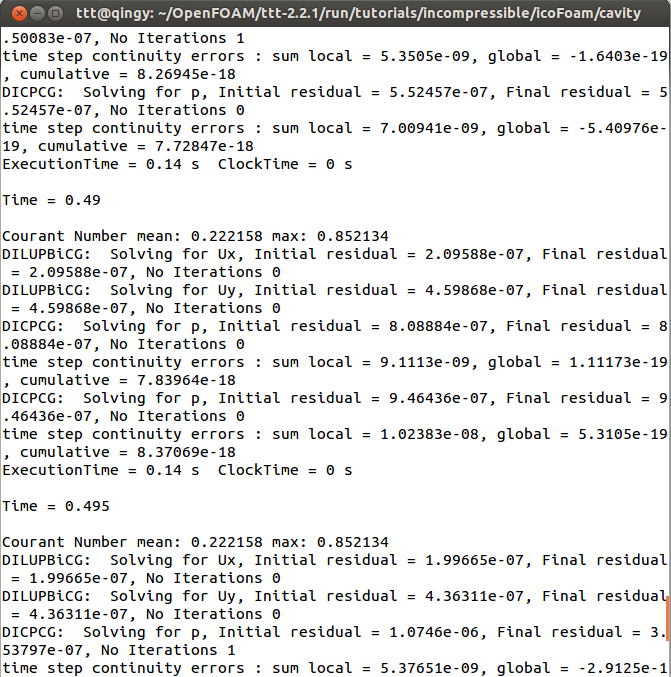
\includegraphics[scale=0.3]{\LocCHonefig/solver.png}
\caption{Iteration on Terminal Window}
\label{solver}
\end{center}  
\end{figure}

\subsection*{Visualization}
To Visualize the results we use Paraview. To open paraview in your terminal type \\
\center \textbf{paraFoam} \\
\flushleft and press $<enter>$. This will open up the paraview window, Fig \ref{pv}.

\begin{figure}[ht]  
\begin{center}  
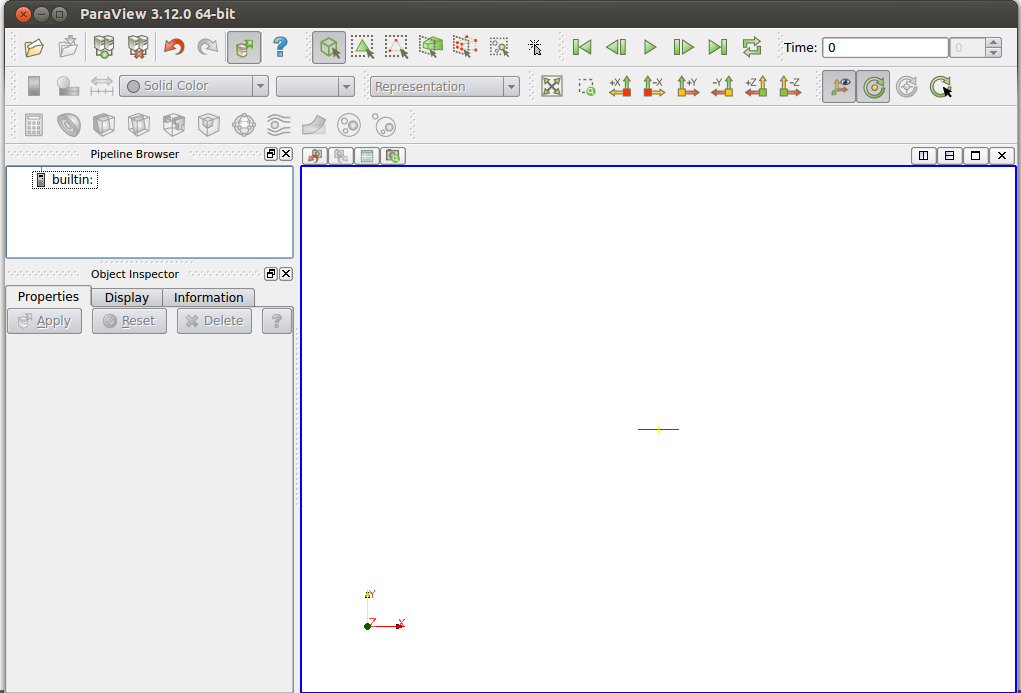
\includegraphics[scale=0.32]{\LocCHonefig/paraview.png}
\caption{Paraview window}
\label{pv}
\end{center}  
\end{figure}

\flushleft Click on the Apply button on the left hand side of the \textbf{Object Inspector} Menu to view the Geometry, Fig\ref{geom}.

\begin{figure}[ht]  
\begin{center}  
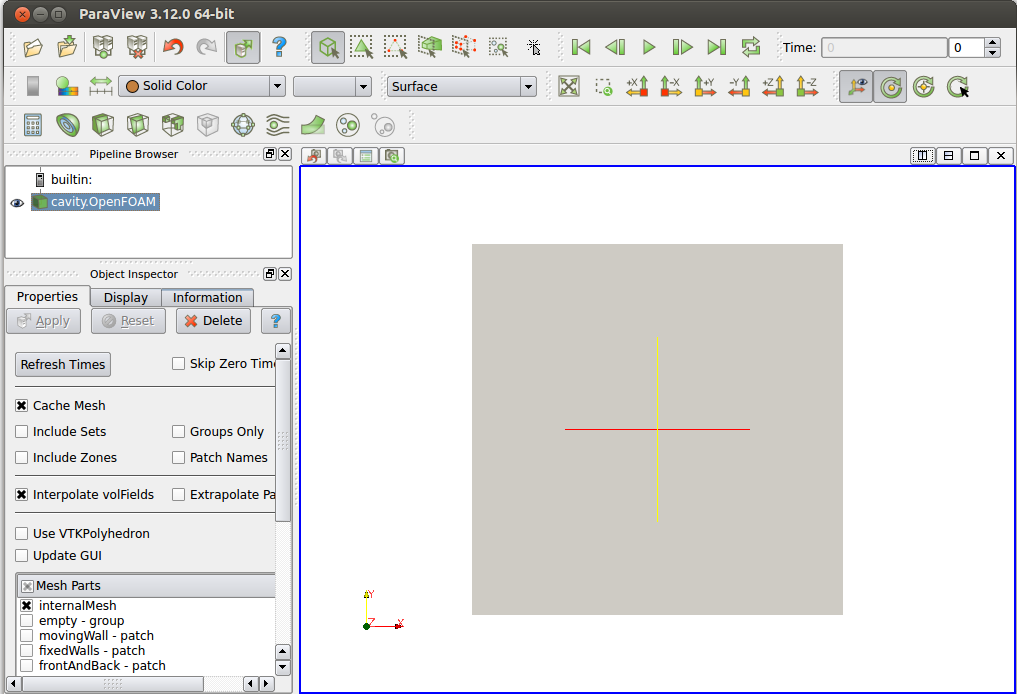
\includegraphics[scale=0.32]{\LocCHonefig/geometry.png}
\caption{Geometry}
\label{geom}
\end{center}  
\end{figure}

\flushleft This brings us to the end of the first chapter. To summaries we have learnt to Install OpenFOAM and Paraview and ran a test example. 
The next chapter will cover about creating simple geometry in OpenFOAM.

\chapter{Creating a Simple Geomtery in OpenFoam}
\thispagestyle{empty}
\label{sec:chap2}
\newcommand{\LocCHtwofig}{\Origin/CHAPTERS/chap2/figures}

In this chapter we will learn how to create a simple geometry in OpenFOAM using the blockMeshDict utility of OpenFOAM. We can create simple geometries
like a square, rectangle , circular cylinder using blockMeshDict.

\section{Geometry creation}
Here we will use the lid-driven cavity problem example mentioned in the previous chapter for the pre-processing. As previously mentioned you can type the following path in the command terminal to open the id-driven cavity problem:
\small{cd OpenFOAM/OpenFOAM-2.3.0/run/tutorials/incompressible/icoFoam/cavity}\newline
\flushleft After this if you type “ls” in the command terminal would see three folder inside it given as:

\begin{itemize}
\item 0
\item constant
\item system
\end{itemize}

\flushleft where the 0 folder gives the initial boundary conditions, constant gives the geomtery file and system folder gives the number of the iterations the solver would run along other important files. You can find the boundary of the problem in a polymesh folder inside constant. In order to open that type the following in the command terminal and then press $<enter>$:
\center \textbf{cd constant/polymesh}
\flushleft Then type ls to in the command terminal and press $<enter>$. This shows the geomtery file given as blockMeshDict file. In order to view this file type the following in the command terminal:

\center \textbf{gedit blockMeshDict}

\flushleft where gedit it the name of the editor we have used. Note that you may use any other text file editor to view and edit this file.
\flushleft Now you can see the gedit window containing the geometry file. In order to draw a geomtery in OpenFoam you need to follow the below mentioned instructions.
\flushleft In openFoam a geomtery is broken down into small blocks and are then numbered starting from 0, as shown in the Fig \ref{geometry}

\begin{figure}[ht]  
\begin{center}  
\includegraphics[scale=0.32]{\LocCHtwofig/geometry1.png}
\caption{geomtery points of the lid driven cavity}
\label{geometry}
\end{center}  
\end{figure}
 
\section{blockMeshDict} 
\flushleft Note that in openFoam to create a 2-D geometry you need to give a unit cell thickness in the Z axis. Now in order to create a new geomtry file open a new folder in destop and rename it a “blockMeshDict”. 
\flushleft A blockMeshDict file basically has the following parts:

\begin{itemize}
\item Foam File details
\item vertices
\item blocks
\item edges
\item boundary
\item mergepatchpairs
\end{itemize}

\flushleft Note that the line convertToMeter gives unit in which the geomtery is drawn. For example, as we are drawing the geomtery in meters for this problem we will keep convertToMeters as 1. Now after opening the new blockMeshDict file created in the desktop copy the lines from initial Foam File till convertToMeters from the old file and paste it. After this type vertices and then you can give the X, Y and Z co-ordinates of the boundary as shown below:

\begin{figure}[ht]  
\begin{center}  
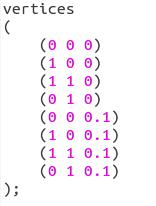
\includegraphics[scale=0.66]{\LocCHtwofig/vertices.png}
\caption{coordinates of boundary geomtery points of the lid driven cavity}
\label{vertices}
\end{center}  
\end{figure}

\flushleft Then type block, inside which you give the details of the boundary co-ordinates along with the number of mesh divisions in X, Y and Z direction in the following way, fig \ref{blocks}:

\begin{figure}[ht]  
\begin{center}  
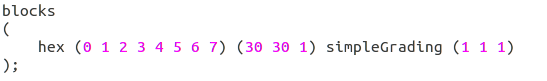
\includegraphics[scale=0.66]{\LocCHtwofig/blocks.png}
\caption{block details of the geomtery}
\label{blocks}
\end{center}  
\end{figure}

\flushleft Here hex represents hexahedral block and the number next to that gives the names of the points at the boundary in clock-wise direction to form a block. Note that for more than one blocks the number of points would be more. The number of grid points can be modified as per requirement. For this problem we have used a 2-D mesh having 30x30 divisions and unit dept. Now since we have all straight edges in this geometry, we will keep the egdes empty.

\begin{figure}[ht]  
\begin{center}  
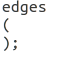
\includegraphics[scale=0.66]{\LocCHtwofig/edges.png}
\caption{edge details of the geomtery}
\label{edges}
\end{center}  
\end{figure}
\vspace{2cm}
\flushleft Next we give the details of the boundary. In the geometry we can see the following boundary conditions,as shown in fig \ref{boundary}:
\begin{itemize}
  \item moving wall
  \item fixed wall
  \item front and back
\end{itemize}
\begin{figure}[ht]  
\begin{center}  
\includegraphics[scale=0.45]{\LocCHtwofig/boundary.png}
\caption{boundary names of the geomtery}
\label{boundary}
\end{center}  
\end{figure}
\flushleft where it has a top moving wall and three fixed wall. The front and back faces are kept empty as this is a 2-D problem. 
\vspace{10cm}
\flushleft Now in the blockMeshDict file you can type the boundary as shown in fig \ref{boundary_name}:
\begin{figure}[ht]  
\begin{center}  
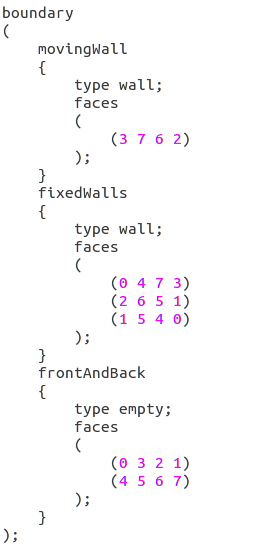
\includegraphics[scale=0.66]{\LocCHtwofig/boundary_name.png}
\caption{boundary details of the geomtery}
\label{boundary_name}
\end{center}  
\end{figure}


\flushleft Here within the boundary names enter the type of boundary used and  then faces, giving the points of the block forming a particular boundary. Note that you should be very careful while writing the order of the points. The order should be such that if you place a folded palm on the surface of a boundary the thumb should be pointing normal to the surface and the fingers should be folded such that they make a curl in clockwise or anti-clockwise direction. Note that you should use either clockwise or anti-clockwise convention throughout the file and but not both. Also you should be very careful regarding openning and closing of brackets in this file.

\flushleft After this$,$ in a new line type mergePatchPairs. Since in this problem we do not have to merge any patches we will keep this empty$,$ fig \ref{merge}.
\vspace{0.32cm}
\begin{figure}[ht]  
\begin{center}  
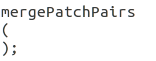
\includegraphics[scale=0.66]{\LocCHtwofig/merge.png}
\caption{merge patch details of the geomtery}
\label{merge}
\end{center}  
\end{figure}

\flushleft Note that two “P”'s are capital here.
\flushleft After completing writing this file save it and close this file. Thus you have learned ho wto create a geomtery file.
\flushleft Now go back to the command terminal and type the following twice to go back to cavity folder:

\center \textbf{cd ..} 

\flushleft Next you can mesh this geomtry by typing blockMesh in the command terminal. After this you can view the geometry by opening paraview. For this type paraFoam in the command terminal and press $<enter>$.
\flushleft In the paraview window press Apply button on the left hand side of the Object Inspector Menu to
view the Geometry, as shown in the fig \ref{paraview1}:
\begin{figure}[ht]  
\begin{center}  
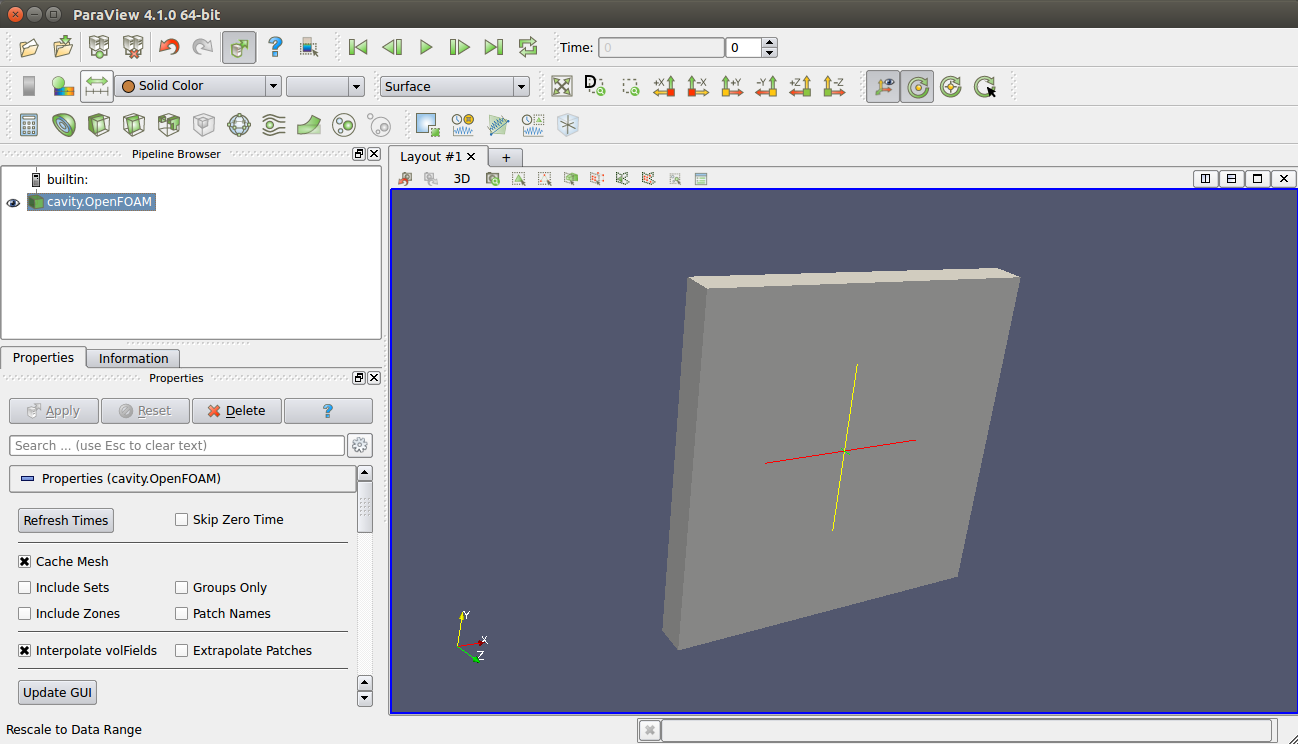
\includegraphics[scale=0.32]{\LocCHtwofig/paraview1.png}
\caption{Paraview window showing the 2-D geometry}
\label{paraview1}
\end{center}  
\end{figure}

\flushleft As you as learned in the previous chapter, you can use different feature in the paraview window to check the details of the geometry.

\chapter{Importing Mesh From Third Party Software in OpenFOAM}
\thispagestyle{empty}
\label{sec:chap3}
\newcommand{\LocCHthreefig}{\Origin/CHAPTERS/chap3/figures}

OpenFOAM can be used for creating and meshing geometrical shapes like Box, Pipe. When dealing with complex geometries like a turbine blade, aircraft,
ship etc, we cannot use the blockMesh utility. In such cases it is always better to create the geometry and mesh in dedicated CAD and Meshing softwares 
and solve those usiing OpenFOAM. As a prerequisite it is expected the user should have knowledge about creating geometry and generating mesh in softwares
like Gmabit, Gmsh, Salome, ICEM etc. This chapter deals with the steps involved in importing mesh files in OpenFOAM using different mesh conversion tools.

\section{Geometry}

We will use the above problem of Flow over a square cylinder as an example for importing mesh file in OpenFOAM. Here we have a square cylinder
of length 1m and height 1 m. Inlet velocity is set at 1 $\frac{m}{s}$ for Reynolds number (Re) 100. The size of the domain choosen is 60 m by 40 m.
The boundary conditions are as shown in the , Fig \ref{square} below.

\begin{figure}[t]  
\centering  
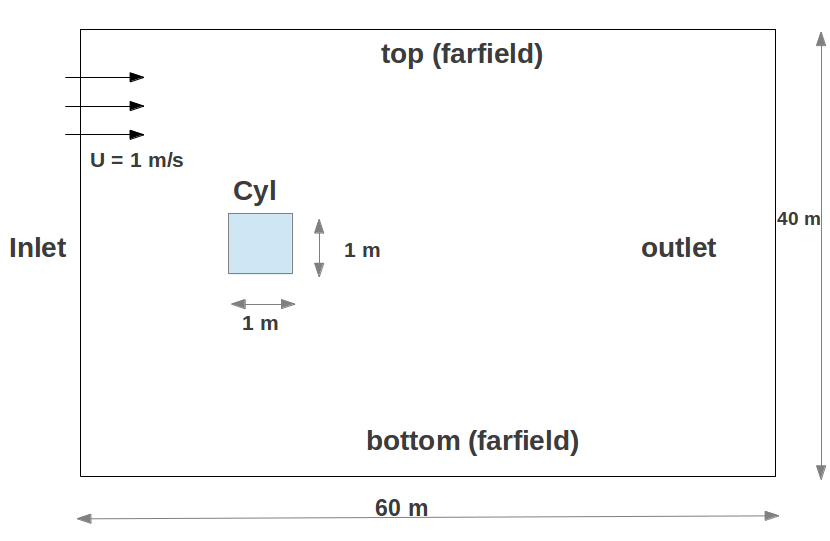
\includegraphics[width=\lgfig]{\LocCHthreefig/square.png}
\caption{Flow over square Cylinder}
\label{square}  
\end{figure}

\section{Meshing}

We have generated a hexhedral mesh for the above geometry with 40000 cells and saved the mesh file as cylmesh.msh. 
The mesh generated is as shown below, Fig \ref{mesh} 

\begin{figure}[h]  
\centering
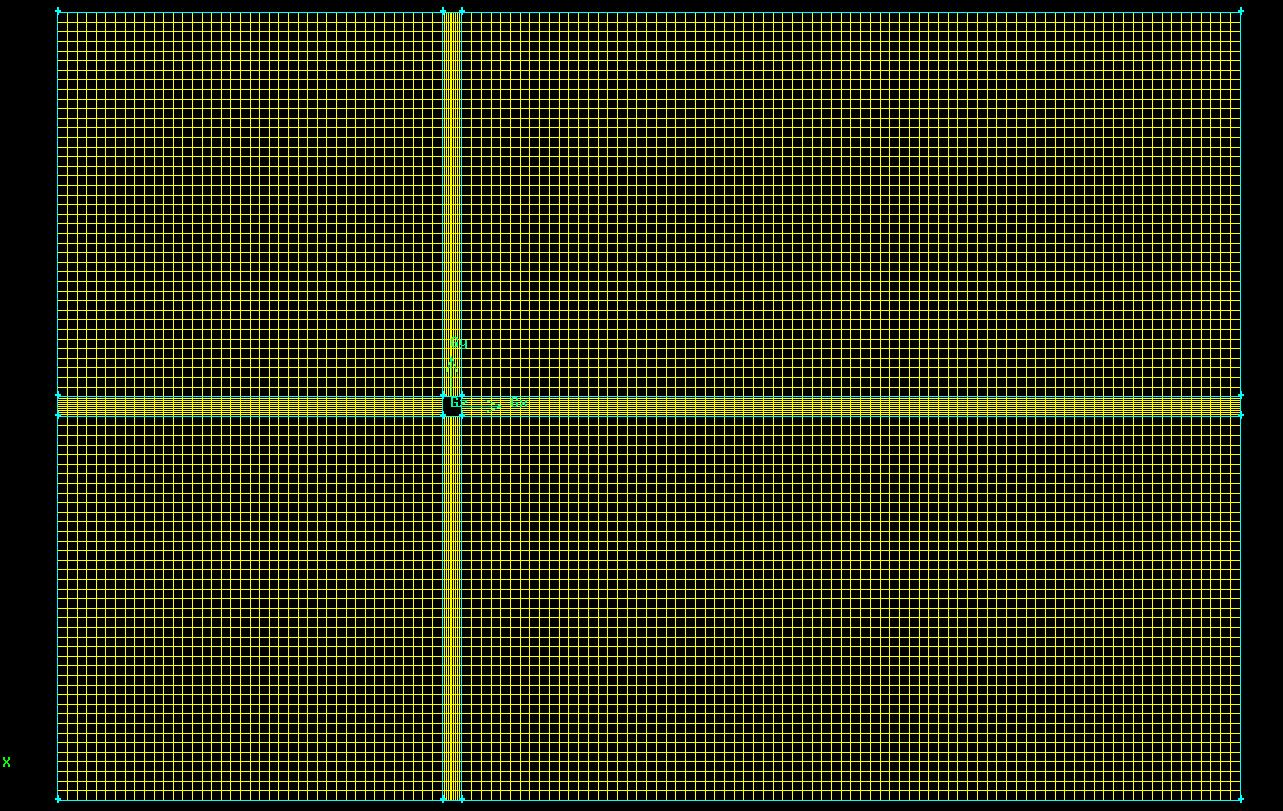
\includegraphics[width=\lgfig]{\LocCHthreefig/cylmesh.jpeg}
\caption{Mesh}
\label{mesh}
  
\end{figure}

\section{Importing the mesh file}

In incompressibel solvers go to icoFoam and create a solver inside it by the name \textbf{cylinder}. Now go inside the cavity case and copy the 
\begin{itemize}
\item 0
\item system
\end{itemize}

\flushleft folder and paste it inside the cylinder folder. Please make a not here that we do not need the \textbf{constant} folder here. After this copy the 
cylmesh.msh mesh file create earlier and paste this inside this folder. Thus the our case file is now ready. Now open the command terminal and type the
path for the cylinder folder. Now since we have a Fluent (.msh) mesh file we will use the mesh conversion command as shown below followed by the file name \\
\centering \textbf{fluentMeshToFoam file-name.msh} \newline

\flushleft In the terminal window type the above command with the file name and press enter.

\begin{figure}[h]  
\centering
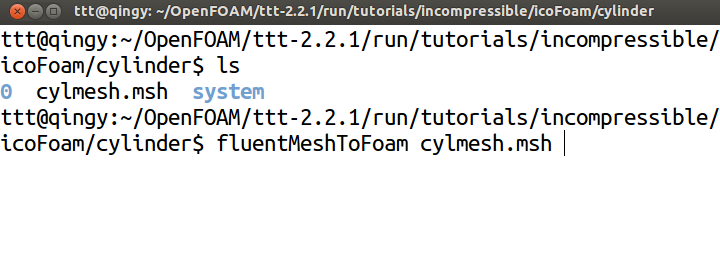
\includegraphics[width=\lgfig]{\LocCHthreefig/conversion.png}
\caption{convert}
\label{mesh}
\end{figure}

\flushleft In case you have a 3D mesh file then you can use the command \\ \vspace{0.5cm}
\centering {\textbf{fluent3DMeshToFoam file-name.msh}} \newline

\flushleft The Fluent mesh file is converted into OpenFOAM mesh file. Now if we look back into our cylinder folder we can see that the "constant"
folder is now generated. When we open the constant folder we will see that the transport properties file is missing. Since we had converted the 
fluent mesh file into openfoam the fluid property files were missing. Copy the transport property file from the constant folder of cavity case
and paste this inside the constant folder of cylinder. The trasnportProperties file contains the value of fluid viscosity, we can either change it
or keep it default. \newline

\flushleft Make a note here that we do not use the \textbf{blockMesh} command here

\section{Boundary Conditions}

When we import the geometry in OpenFOAM we need to be very careful with the boudnary names used while creating the mesh file. Since OpenFOAM is case
sensitive in case of any mistake with the boundary names can create an error while running the solver. To view the boundary names in the command terminal
go to polyMesh folder inside the constant. Inside polyMesh you can see a file by the name \textbf{boundary}. Open this file in any editor of your
choice, eg, gedit boundary, Fig \ref{boundary}.

\begin{figure}[h]  
\centering
\includegraphics[width=\lgfig]{\LocCHthreefig/boundary.png}
\caption{Boundary file}
\label{boundary}
\end{figure}

\flushleft The boundary names will be as shown in the domain shown above, Fig \ref{square}. In case of any error with the boundary names you can
always refer to this boundary file. Now in your command terminal go to the 0 folder and open the pressure file. Make sure that the boundary names 
match exactly the names in the boundary file, in case of errors make the necessary changes.

\section{Solver settings}

In the terminal window go to the controlDict file inside system and open it in any editor of your choice. Change the endTime from 0.5 to 1.5 seconds.
Save the file and close it, Fig \ref{cd} and come back to the cylinder folder.

\begin{figure}[h]  
\centering
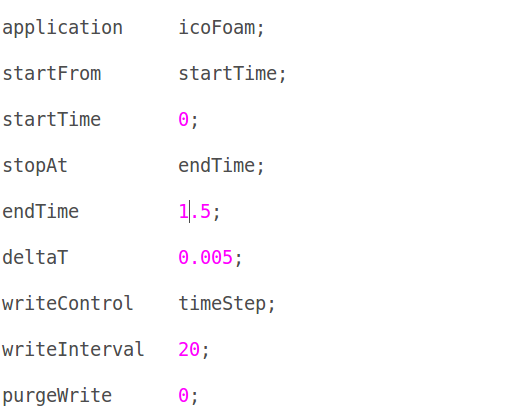
\includegraphics[width=\lgfig]{\LocCHthreefig/controldict.png}
\caption{controlDict file}
\label{cd}
\end{figure}

\flushleft After making the necessary changes we can now run the solver. In the temrinal window type the name of the solver \textbf{icoFoam}
and press enter. The iterations will be seen running on the terminal window. After the iterations stop we can now start with the visualization.

\section{Post-Processing}

Launch paraview by typing \textbf{paraFoam} in the terminal window and once it opens click on the Apply button to view the geometry, Fig \ref{geom}.
In the active varialble control menu change from Solid Color to Velocity (U). You can now see the initial conditions for velocity, Fig \ref{vel}.
To view the animation on the right hand top of paraview click on the play button of VCR menu. You can see the change in velocity in the paraview 
window with the passage of time, Fig \ref {vel-1}.

\begin{figure}[h]  
\centering
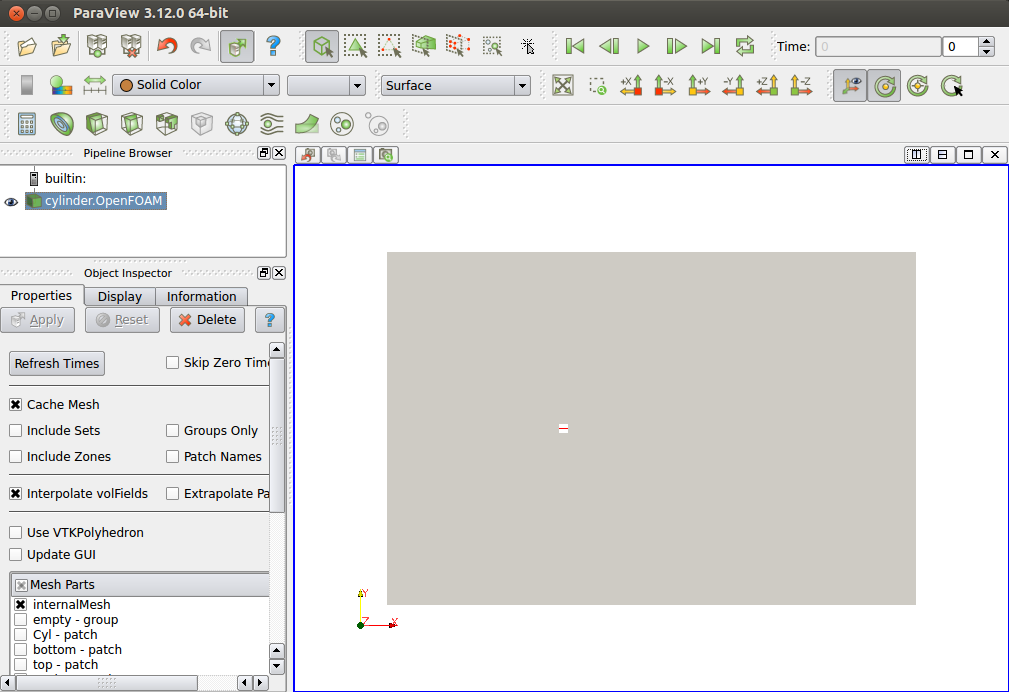
\includegraphics[width=\lgfig]{\LocCHthreefig/geom-paraview.png}
\caption{Geometry in Paraview}
\label{geom}
\end{figure}

\begin{figure}[h]  
\centering
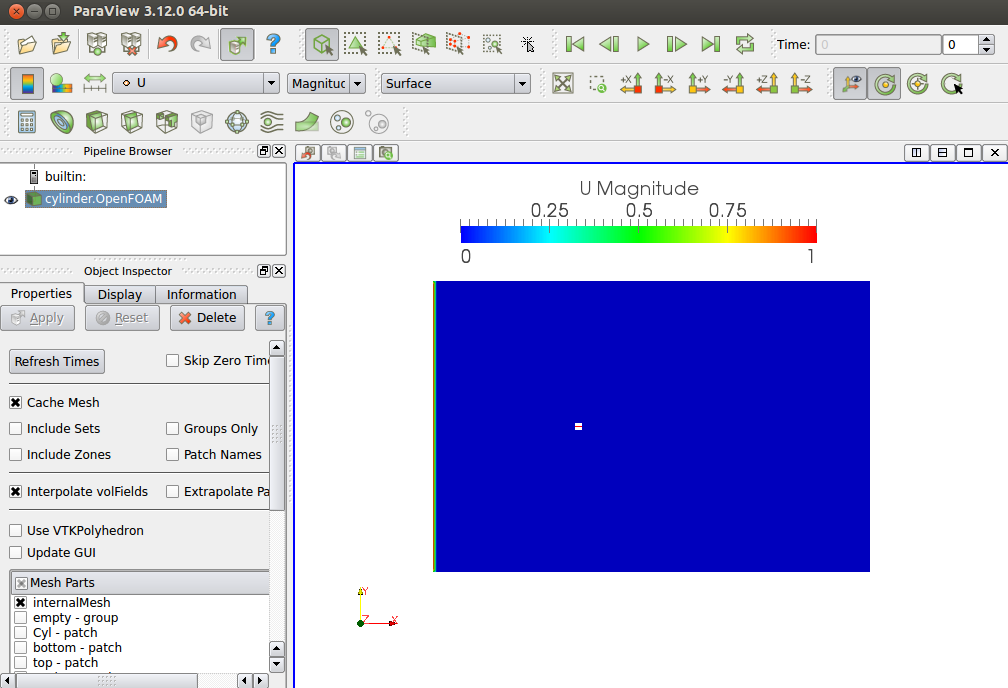
\includegraphics[width=\lgfig]{\LocCHthreefig/vel.png}
\caption{Initial velocity condition}
\label{vel}
\end{figure}

\begin{figure}[h]  
\centering
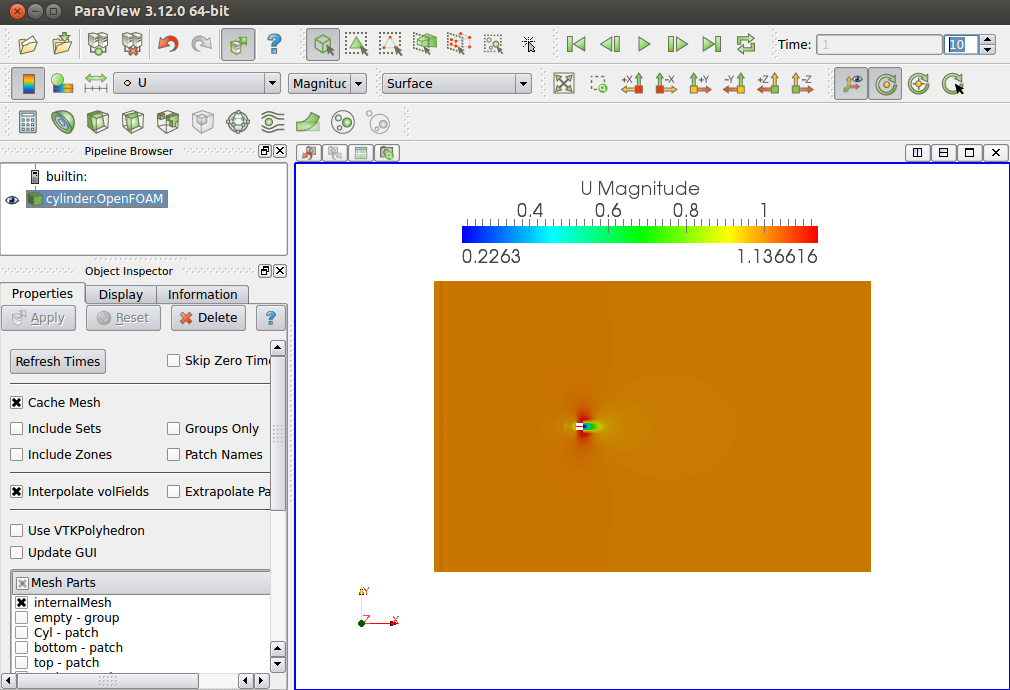
\includegraphics[width=\lgfig]{\LocCHthreefig/vel-1.png}
\caption{Velocity at 1 sec}
\label{vel-1}
\end{figure}

\section{Mesh Conversion Commands}

The user can also import mesh files from other meshing softwares as well. Here is a list of commands to import mesh files in OpenFOAM.

\begin{itemize}
\item ANSYS : ansysToFoam file-name
\item IDEAS : ideasToFoam file-name
\item CFX : cfxToFoam file-name
\item SALOME : ideasUnvToFoam file-name
\end{itemize}




\chapter{Installing and Running Gmsh}
\thispagestyle{empty}
\label{sec:chap4}
\newcommand{\LocCHfourfig}{\Origin/CHAPTERS/chap4/figures}

Gmsh is a Free and Open Source three dimensional finite element grid generator with a build-in CAD engine and post-
processor. There are four modules available in Gmsh such as Geometry, Meshing, Solver and Post-Processiing. Using
Gmsh we can mesh the geometry and import it in OpenFOAM using the mesh conversion utilities (see chapter 17 for more info).
In this chapter we will cover how to install Gmsh and create a simple geometry.It is expected that the user should have knowledge 
about Meshing.

\section{Installing Gmsh}

Gmsh can be installed using Synaptic Package Manager. Open Gmsh in your system by typing your system passowrd.
In the search box type Gmsh and install it, Fig \ref{synaptic-gmsh}. This might take some time depending on your internet speed.

\begin{figure}[ht]  
\begin{center}  
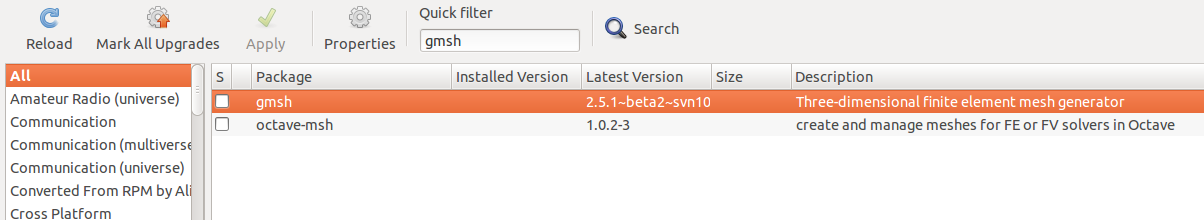
\includegraphics[scale=0.32]{\LocCHfourfig/synaptic-gmsh.png}
\caption{Install Gmsh}
\label{synaptic-gmsh}
\end{center}  
\end{figure}


\flushleft Alternately we can also install Gmsh from the gmsh website given below,

\center {\textbf{http://geuz.org/gmsh/}} \newline

\flushleft Open this website in your browser and scroll down to download. Now Download Gmsh according to the given current stable release 
Fig \ref{download-gmsh} according to your Operating System (OS).

\begin{figure}[ht]  
\begin{center}  
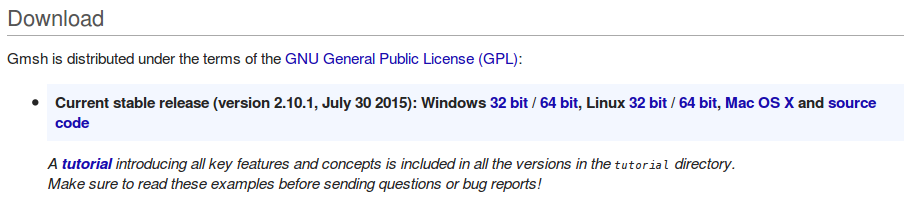
\includegraphics[scale=0.352]{\LocCHfourfig/download-gmsh.png}
\caption{Download stable release}
\label{download-gmsh}
\end{center}  
\end{figure}

\begin{figure}[ht]  
\begin{center}  
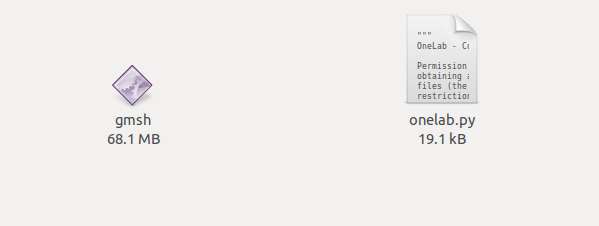
\includegraphics[scale=0.26]{\LocCHfourfig/gmsh-icon.png}
\caption{gmsh-icon}
\label{gmsh-icon}
\end{center}  
\end{figure}


\flushleft In the Download folder extract the downloaded gmsh tar file. After you open the folder you will see folder named bin, click on it. 
Inide the bin folder you will see the Gmsh icon, Fig \ref{gmsh-icon}. Double click on it to launch the Gmsh Start screen, Fig \ref{gmsh-start} \newline

As a pracice to learn Gmsh we will create a cube of sides 1 unit as seen in the Fig, \ref{geometry1}. On the left hand side in the Gmsh window you can 
see three modules namely,

\begin{itemize}
\item Geometry
\item Mesh
\item Solver
\end{itemize}

Click on the Geometry module, then go to Elementary Entities, inside elementary entities go to add and then click on points. This will open up a
window where you can enter the X, Y and Z co-ordinates starting with 0 inside each box and press Enter, Fig \ref{point}. Now
enter points for all the remaining 7 vertices to complete the cube, Fig \ref{geometry1}. In the Gmsh screen we can see the eight points, you can move those points
using the left mouse click. To join these points click on Straight-line option under Elementary Entities. Now select any two points to create a straight line, click 
on the start point and then the second point to create a line. Similarly join all the other points to create a cube as shown in the Fig, \ref{line} below.
As you can see on the Gmsh screen you can press e to end selection and q to abort.

\begin{figure}[t]  
\begin{center}  
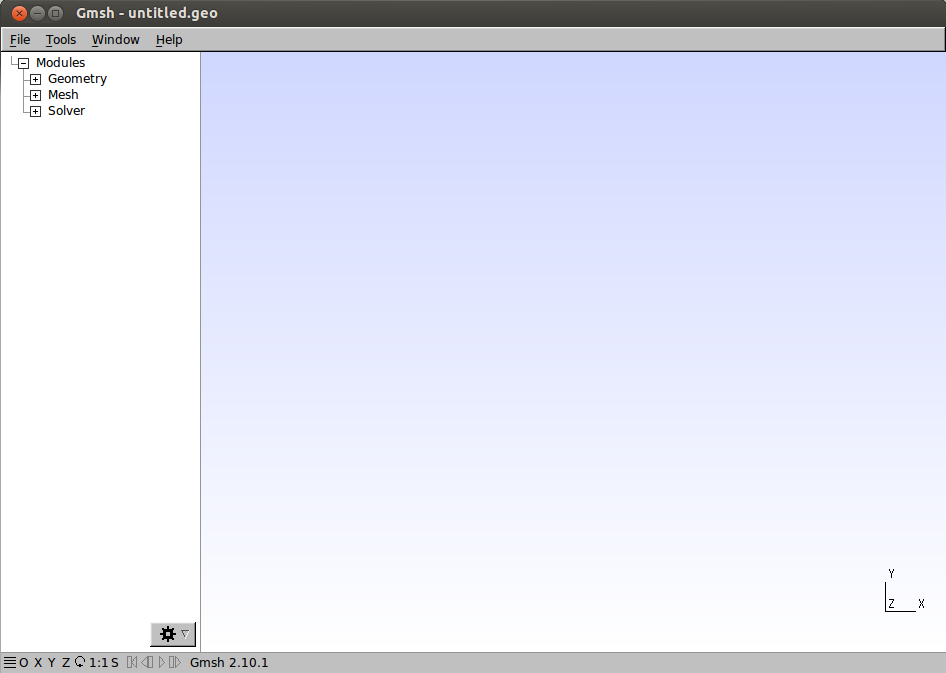
\includegraphics[scale=0.28]{\LocCHfourfig/gmsh-start.png}
\caption{gmsh-icon}
\label{gmsh-start}
\end{center}  
\end{figure}

\begin{figure}[t]  
\begin{center}  
\includegraphics[scale=0.28]{\LocCHfourfig/geometry1.png}
\caption{Cube of unit dimension}
\label{geometry1}
\end{center}  
\end{figure}

\begin{figure}[t]  
\begin{center}  
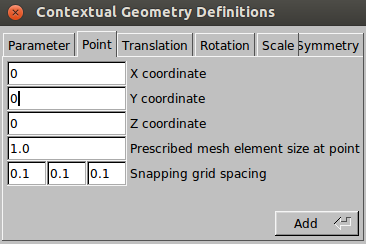
\includegraphics[scale=0.28]{\LocCHfourfig/point-gmsh.png}
\caption{Points window}
\label{point}
\end{center}  
\end{figure}

\begin{figure}[t]  
\begin{center}  
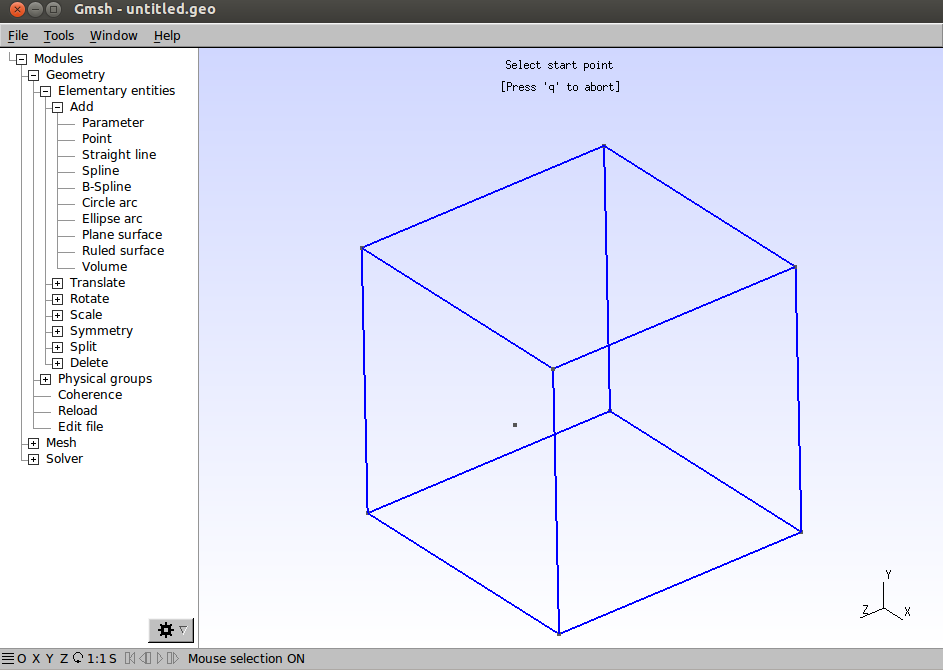
\includegraphics[scale=0.28]{\LocCHfourfig/cube-gmsh.png}
\caption{Join the points using line}
\label{line}
\end{center}  
\end{figure}

\subsection{Create Faces}

To create faces for the cube click on plane-surface unde elementery enetities. After this select the outer booundaries of the face of a rectangle.
Select the edges of the bottom face first.Once you select the edges they will turn red in color, Fig \ref{face}. Check in case if there is any hole in the 
face, if none then press e to end selection. You will notice that a face will appear with dasshed center lines, Fig \ref{cl}. Repeat this procedure for 
remaining faces, Fig \ref{face-all} and finally press q to abort.

\begin{figure}[t]  
\begin{center}  
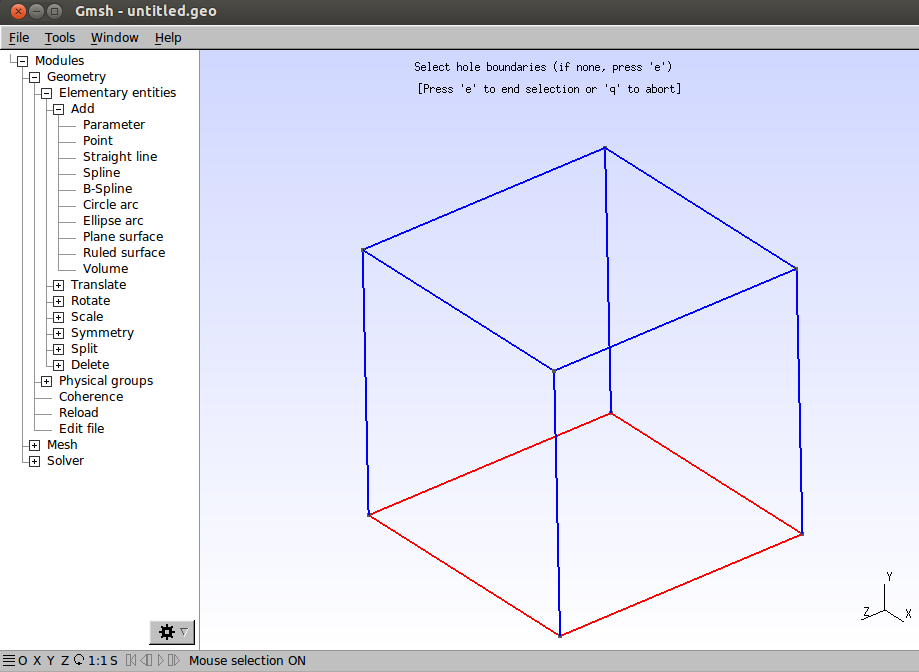
\includegraphics[scale=0.28]{\LocCHfourfig/face-red.png}
\caption{Selct edges}
\label{face}
\end{center}  
\end{figure}


\begin{figure}[t]  
\begin{center}  
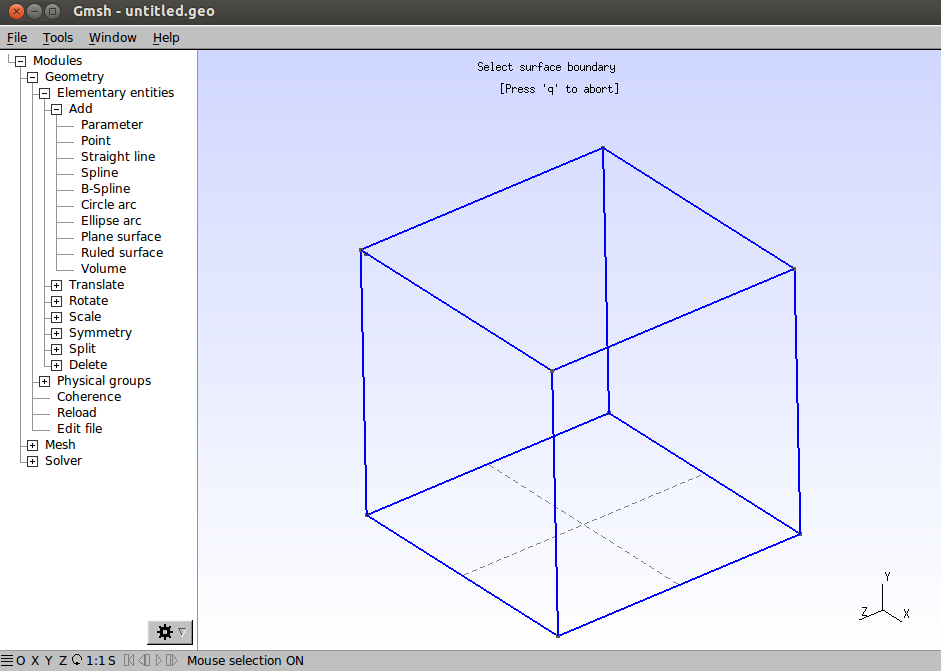
\includegraphics[scale=0.28]{\LocCHfourfig/face-cl.png}
\caption{Bottom Face}
\label{cl}
\end{center}  
\end{figure}

\begin{figure}[t]  
\begin{center}  
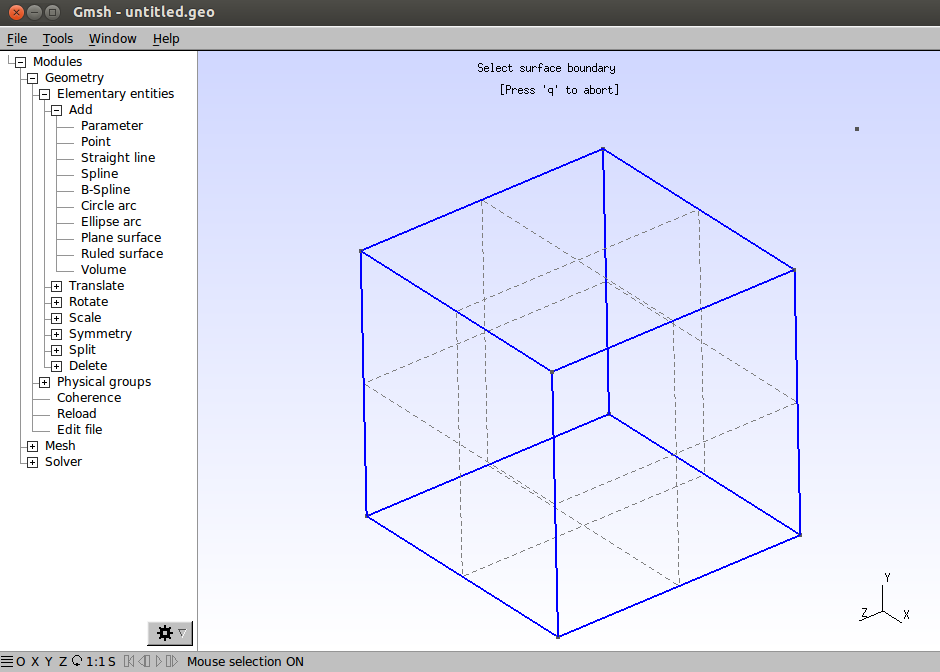
\includegraphics[scale=0.28]{\LocCHfourfig/face-all.png}
\caption{Create faces for all surfaces}
\label{face-all}
\end{center}  
\end{figure}

\subsection{Creating Volume}

We now need to create volume boundary. We need to select the Volume boundary similar to selecting boundary for faces. 
Click on the Volume boundary under elementery entities and click on boundary surface of the cube and press e to end selection. A yellow dot will
appear at the center of the cube which represents volume in Gmsh. Press q to abort the selction.

\begin{figure}[t]  
\begin{center}  
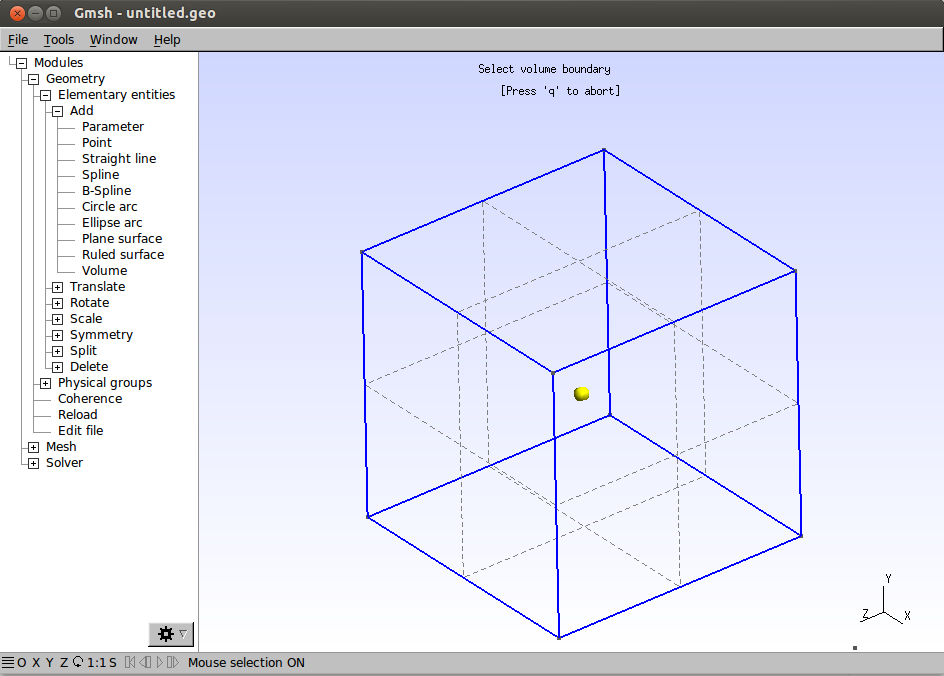
\includegraphics[scale=0.28]{\LocCHfourfig/vol-gmsh.png}
\caption{Volume}
\label{vol}
\end{center}  
\end{figure}

\subsection{Physical Groups}

In Gmsh we need to create physical groups which will be useful for exporting the Mesh file to OpenFOAM. To do so click on Physical Group under Geometry Module.
Click on Add and then Surface. Upon selection of any face it will turn red. Now press e to end selection. Do this procedure for all the remaining faces
and press q to abort. Also we need to select the Physical Volume. Click on Volume under Physical Groups and select the yellow dot at the center of the cube.
The yellow dot will turn red in colora dn press e to end selection and q to abort.

To save the geometry under the file menu click on Save as and save the geometry by the name cube.geo. Here "geo" stands for geometry. Click OK twice
to save the geometry. 



\chapter{Downloading and Installing Salome}
\thispagestyle{empty}
\label{sec:chap5}
\newcommand{\LocCHfivefig}{\Origin/CHAPTERS/chap5/figures}

Salome is a Free and Open Source  CAD (Computer Aided Drawing), Meshing and Visualization Software for Numerical simulation. 
We can Create/modify, import/export (IGES, STEP, BREP), repair/clean CAD models and Mesh CAD models, edit mesh, check mesh quality, 
import/export mesh (MED, UNV, DAT, STL) using Salome. In this chapter we will learn how to download and intall Salome in any Operating system.

\section{Download Salome}

Open your browser and in the address bar type the url given below, \newline

\centering \textbf{www.salome-platform.org} \newline

\flushleft To Download Salome the user needs to create a account on the salome site. To do this on the left hand side of the salome screen website
scroll down to the bottom of the \textbf{Navigation} bar, Fig \ref{navi}, where you can see the new user option. Click on it and enter the required
personal details. \newline
\flushleft After you enter the details click on the register button at the bottom as shown in, Fig \ref{details}. Once done you will be directed 
to a screen showing that you have been registered. This also states thatv once you have done with registration you have to login to your email. Now 
open the mail sent by Salome and click on the link shown in Fig, \ref{link}. This link will direct you to a window where you need to set your password
for your Salome account. Enter the password and confirm it and press set my password button, Fig \ref{pass}. After this it will direct you to a window
which says your password has been set successfully. You may now login with your username and password. \newline

\flushleft In the Navigation bar click on Downloads after which you will be directed to a page which will show various bianaries for various Linux
distributions. You can choose according to your Operating System and 32/64 bit size. Since in this book we are working on a 64 bit platform we
will download Linux Debian 7 64-bits or Ubuntu 14.04 64-bits binary, Fig \ref{binary}. Click on it and Save the file. Since the file size is big it will take some time to download.
After this scroll down to Universal Binaries and click on the \textbf{Linux 64-bits} to download it. Note that 32-bit version of binaries are no
more supported for the latest version of Salome.

\begin{figure}[h]  
\centering
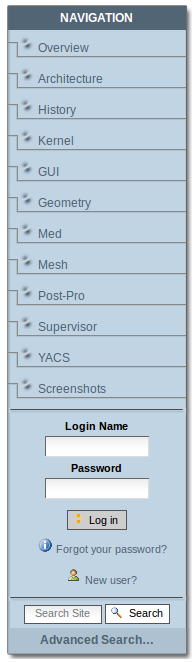
\includegraphics[scale=0.3]{\LocCHfivefig/navi.png}
\caption{Navigation Bar}
\label{navi}
\end{figure}

\begin{figure}[h]  
\centering
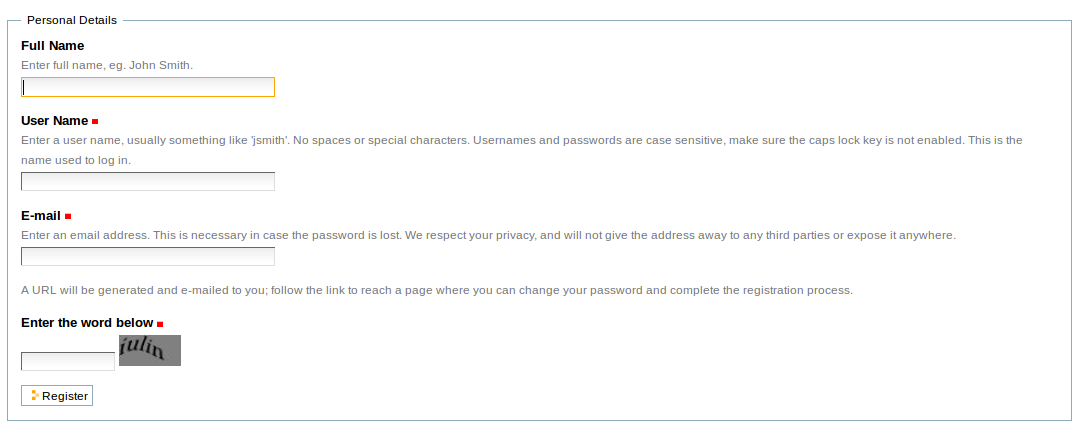
\includegraphics[scale=0.32]{\LocCHfivefig/details.png}
\caption{User Details}
\label{details}
\end{figure}

\begin{figure}[h]  
\centering
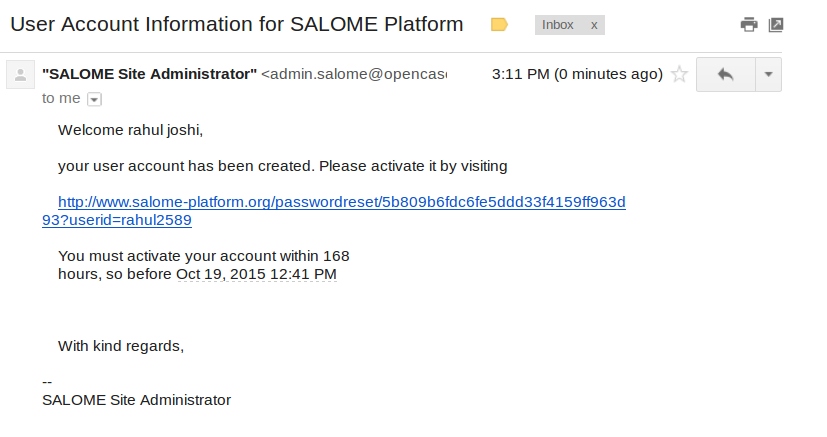
\includegraphics[scale=0.35]{\LocCHfivefig/link.png}
\caption{Salome Link}
\label{link}
\end{figure}

\begin{figure}[h]  
\centering
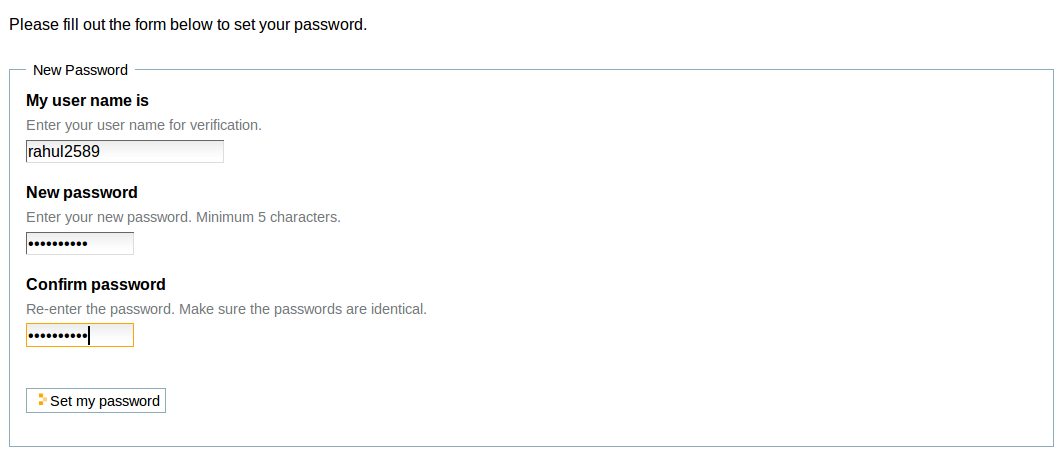
\includegraphics[scale=0.35]{\LocCHfivefig/pass.png}
\caption{Enter Password}
\label{pass}
\end{figure}

\begin{figure}[h]  
\centering
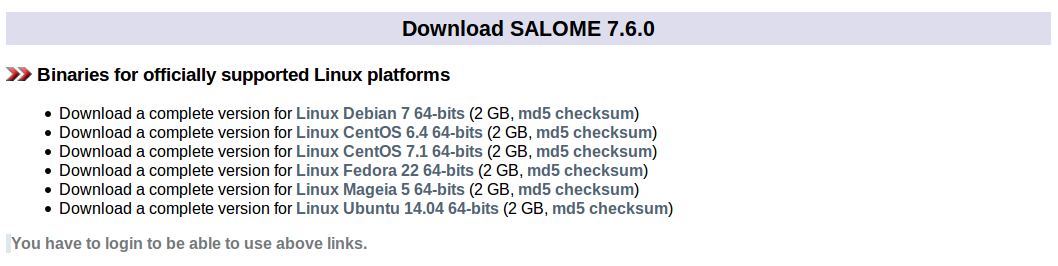
\includegraphics[scale=0.35]{\LocCHfivefig/binary.png}
\caption{Salome Linux Debain 7 64 bit binary}
\label{binary}
\end{figure}

\begin{figure}[h]  
\centering
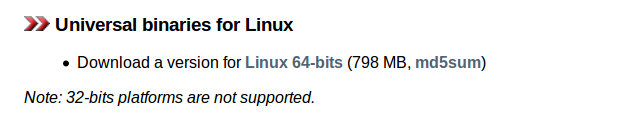
\includegraphics[scale=0.45]{\LocCHfivefig/universal.png}
\caption{Universal Binaries}
\label{univ}
\end{figure}

\section{Installing Salome}

The downloaded files are saved in the Download folder. Open the Download folder in your system and check for both the tar file and a self-extracting file.
Copy these two files and in your home folder create a new folder by the name Salome and paste these two files inside it, Fig \ref{download}.



\chapter{}
\thispagestyle{empty}
\label{sec:chap6}
\newcommand{\LocCHsixfig}{\Origin/CHAPTERS/chap3/figures}





%\input{user-code/sw-env/sw-env.tex}
%\input{user-code/led/led.tex}
%\input{user-code/push/push.tex}
%\input{user-code/ldr/ldr.tex}
%\input{user-code/dcmotor/dcmotor.tex}
%\input{user-code/pot/pot.tex}
%\input{user-code/servo/servo.tex}
%\input{texfiles/servo.tex}
%\input{texfiles/Appendix.tex}
%\appendix
%\input{texfiles/sp-appendix.tex}
%\input{windows/windows}

%\bibliography{bibliography.bib}
%\printindex
%\input{texfiles/AuthorInfo.tex}
\end{document}